\begin{bt}%[9D6H18-2]
% nguon: Cụm 11 – Đề tham khảo Tuyển sinh 10 năm học 2026-2027 TP.HCM – Đề số 33
Cho hàm số $y = \dfrac{1}{3}x^2$ có đồ thị là parabol $(P)$.
\begin{enumerate}[a)]
    \item Vẽ đồ thị $(P)$ trên mặt phẳng tọa độ $Oxy$.
    \item Tìm tọa độ các điểm thuộc $(P)$ sao cho hoành độ và tung độ của điểm đó đối nhau.
\end{enumerate}
\loigiai{
\begin{enumerate}[a)]
    \item Bảng giá trị:
    \begin{center}
    \begin{tabular}{|c|c|c|c|c|c|}
    \hline
    $x$ & $-6$ & $-3$ & $0$ & $3$ & $6$ \\ \hline
    $y = \dfrac{1}{3}x^2$ & $12$ & $3$ & $0$ & $3$ & $12$ \\ \hline
    \end{tabular}
    \end{center}
    Đồ thị parabol $(P)$ đi qua gốc tọa độ $O(0;0)$ và các điểm $(-6;12)$, $(-3;3)$, $(3;3)$, $(6;12)$.
    \begin{center}
    \begin{tikzpicture}[>=stealth,scale=0.7]
        \draw[->] (-7,0) -- (7,0) node[below] {$x$};
        \draw[->] (0,-1) -- (0,13) node[left] {$y$};
        \node[below left] at (0,0) {$O$};
        \draw[dashed] (-6,0) node[below] {$-6$} -- (-6,12) -- (6,12) -- (6,0) node[below] {$6$};
        \draw[dashed] (-3,0) node[below] {$-3$} -- (-3,3) -- (3,3) -- (3,0) node[below] {$3$};
        \draw[dashed] (-6,12) -- (0,12) node[left] {$12$};
        \draw[dashed] (-3,3) -- (0,3) node[left] {$3$};
        \draw[thick,smooth,samples=100,domain=-6.2:6.2] plot(\x,{(1/3)*(\x)^2});
        \fill (-6,12) circle (1.5pt) (-3,3) circle (1.5pt) (0,0) circle (1.5pt) (3,3) circle (1.5pt) (6,12) circle (1.5pt);
    \end{tikzpicture}
    \end{center}
    \item Điểm thuộc $(P)$ có hoành độ và tung độ đối nhau nên thỏa mãn $y = -x$.\\
    Ta có phương trình hoành độ giao điểm:
    $$-x = \dfrac{1}{3}x^2 \iff \dfrac{1}{3}x^2 + x = 0 \iff x(x + 3) = 0 \iff \left[\begin{aligned} &x = 0 \\ &x = -3. \end{aligned}\right.$$
    \begin{itemize}
        \item Với $x = 0 \implies y = 0$.
        \item Với $x = -3 \implies y = -(-3) = 3$.
    \end{itemize}
    Vậy tọa độ các điểm cần tìm là $(0;0)$ và $(-3;3)$.
\end{enumerate}
}
\end{bt}

\begin{bt}%[9D6H20-2]
% nguon: Cụm 11 – Đề tham khảo Tuyển sinh 10 năm học 2026-2027 TP.HCM – Đề số 33
Cho phương trình $-5x^2 + 3x + 4 = 0$.
\begin{enumerate}[a)]
    \item Chứng minh phương trình trên luôn có hai nghiệm phân biệt $x_1, x_2$.
    \item Không giải phương trình, hãy tính giá trị của biểu thức:
    $$A = \dfrac{2x_1}{x_2} + \dfrac{2x_2}{x_1}.$$
\end{enumerate}
\loigiai{
\begin{enumerate}[a)]
    \item Phương trình $-5x^2 + 3x + 4 = 0$ có $a = -5, b = 3, c = 4$.\\
    Ta có $\Delta = 3^2 - 4 \cdot (-5) \cdot 4 = 9 + 80 = 89 > 0$.\\
    Vì $\Delta > 0$ nên phương trình có hai nghiệm phân biệt $x_1, x_2$.
    \item Theo định lý Vi-ét, ta có:
    $$\begin{cases} x_1 + x_2 = -\dfrac{b}{a} = \dfrac{3}{5} \\ x_1 x_2 = \dfrac{c}{a} = -\dfrac{4}{5}. \end{cases}$$
    Ta có:
    $$x_1^2 + x_2^2 = (x_1 + x_2)^2 - 2x_1 x_2 = \left(\dfrac{3}{5}\right)^2 - 2 \cdot \left(-\dfrac{4}{5}\right) = \dfrac{9}{25} + \dfrac{8}{5} = \dfrac{49}{25}.$$
    Biến đổi biểu thức $A$:
    $$A = 2\left(\dfrac{x_1}{x_2} + \dfrac{x_2}{x_1}\right) = 2 \cdot \dfrac{x_1^2 + x_2^2}{x_1 x_2}.$$
    Thay các giá trị vào biểu thức $A$, ta được:
    $$A = 2 \cdot \dfrac{\dfrac{49}{25}}{-\dfrac{4}{5}} = 2 \cdot \left(-\dfrac{49}{25} \cdot \dfrac{5}{4}\right) = 2 \cdot \left(-\dfrac{49}{20}\right) = -\dfrac{49}{10}.$$
\end{enumerate}
}
\end{bt}

\begin{bt}%[9D8H26-3]
% nguon: Cụm 11 – Đề tham khảo Tuyển sinh 10 năm học 2026-2027 TP.HCM – Đề số 33
Trong một lớp học có $40$ học sinh, kết quả học tập môn Toán được xếp loại như sau: Giỏi có $8$ học sinh; Khá có $14$ học sinh; Đạt có $12$ học sinh; Chưa đạt có $6$ học sinh.
\begin{enumerate}[a)]
    \item Tính tỉ lệ phần trăm học sinh ở mỗi mức xếp loại học lực.
    \item Chọn ngẫu nhiên $1$ học sinh trong lớp. Tính xác suất của biến cố $A$: ``Học sinh được chọn thuộc loại Khá hoặc Giỏi''.
    \item Chọn ngẫu nhiên $1$ học sinh trong lớp. Biết rằng học sinh được chọn không thuộc loại Chưa đạt, tính xác suất của biến cố $B$: ``Học sinh đó thuộc loại Giỏi''.
\end{enumerate}
\loigiai{
\begin{enumerate}[a)]
    \item Tỉ lệ phần trăm học sinh ở từng mức xếp loại là:
    \begin{itemize}
        \item Loại Giỏi: $\dfrac{8}{40} \cdot 100\% = 20\%$.
        \item Loại Khá: $\dfrac{14}{40} \cdot 100\% = 35\%$.
        \item Loại Đạt: $\dfrac{12}{40} \cdot 100\% = 30\%$.
        \item Loại Chưa đạt: $\dfrac{6}{40} \cdot 100\% = 15\%$.
    \end{itemize}
    \item Không gian mẫu có số phần tử là $n(\Omega) = 40$.\\
    Số học sinh thuộc loại Khá hoặc Giỏi là $14 + 8 = 22$ (học sinh).\\
    Xác suất của biến cố $A$ là:
    $$P(A) = \dfrac{22}{40} = \dfrac{11}{20}.$$
    \item Vì học sinh được chọn không thuộc loại Chưa đạt nên số kết quả có thể xảy ra là:
    $$n(\Omega') = 40 - 6 = 34.$$
    Số học sinh thuộc loại Giỏi là $8$ học sinh.\\
    Xác suất của biến cố $B$ trong điều kiện này là:
    $$P(B) = \dfrac{8}{34} = \dfrac{4}{17}.$$
\end{enumerate}
}
\end{bt}

\begin{bt}%[9D6V21-3]
% nguon: Cụm 11 – Đề tham khảo Tuyển sinh 10 năm học 2026-2027 TP.HCM – Đề số 33
Anh Ba có một khu đất hình chữ nhật. Anh dự định dành một phần đất hình vuông cạnh $x\text{ (m)}$ ($x > 0$) ở một góc để trồng cây, phần đất còn lại dùng để lát gạch. Biết chiều dài khu đất hình chữ nhật hơn cạnh hình vuông trồng cây là $7\text{ m}$, và chiều rộng hơn là $3\text{ m}$.
\begin{enumerate}[a)]
    \item Lập biểu thức theo $x$ tính diện tích phần đất dùng để lát gạch.
    \item Biết diện tích phần đất lát gạch là $51\text{ m}^2$, hãy tính chu vi của khu đất trồng cây.
\end{enumerate}
\loigiai{
\begin{enumerate}[a)]
    \item Chiều dài của khu đất hình chữ nhật là: $x + 7\text{ (m)}$.\\
    Chiều rộng của khu đất hình chữ nhật là: $x + 3\text{ (m)}$.\\
    Diện tích toàn bộ khu đất hình chữ nhật là:
    $$S_{\text{khu đất}} = (x + 7)(x + 3)\text{ (m}^2\text{)}.$$
    Diện tích phần đất hình vuông trồng cây là:
    $$S_{\text{cây}} = x^2\text{ (m}^2\text{)}.$$
    Biểu thức diện tích phần đất lát gạch theo $x$ là:
    $$S_{\text{gạch}} = S_{\text{khu đất}} - S_{\text{cây}} = (x + 7)(x + 3) - x^2 = x^2 + 10x + 21 - x^2 = 10x + 21\text{ (m}^2\text{)}.$$
    \item Theo đề bài, diện tích phần đất lát gạch là $51\text{ m}^2$, nên ta có phương trình:
    $$10x + 21 = 51 \iff 10x = 30 \iff x = 3\text{ (thỏa mãn } x > 0\text{)}.$$
    Cạnh của khu đất hình vuông trồng cây là $3\text{ m}$.\\
    Chu vi của khu đất trồng cây là:
    $$C = 4 \cdot 3 = 12\text{ (m)}.$$
\end{enumerate}
}
\end{bt}

\begin{bt}%[9H0V31-3]
% nguon: Cụm 11 – Đề tham khảo Tuyển sinh 10 năm học 2026-2027 TP.HCM – Đề số 33
Một bồn chứa nước gồm hai phần ghép liền nhau: phần dưới là hình trụ có bán kính đáy $r = 1{,}5\text{ m}$, chiều cao $h\text{ (m)}$; phần trên là hình nón có chung đáy với hình trụ, chiều cao của hình nón là $\dfrac{h}{2}\text{ (m)}$.
\begin{enumerate}[a)]
    \item Viết biểu thức thể tích $V$ của bồn chứa nước theo $h$.
    \item Biết thể tích bồn chứa là $V = 9\pi\text{ (m}^3\text{)}$. Người ta sơn toàn bộ mặt ngoài của bồn chứa (không sơn mặt đáy dưới). Tính diện tích cần sơn của bồn chứa (làm tròn kết quả đến hàng đơn vị).
\end{enumerate}
\loigiai{
\begin{enumerate}[a)]
    \item Thể tích phần hình trụ là:
    $$V_{\text{trụ}} = \pi r^2 h = \pi \cdot (1{,}5)^2 \cdot h = \dfrac{9}{4}\pi h\text{ (m}^3\text{)}.$$
    Thể tích phần hình nón là:
    $$V_{\text{nón}} = \dfrac{1}{3}\pi r^2 \cdot \dfrac{h}{2} = \dfrac{1}{3}\pi \cdot (1{,}5)^2 \cdot \dfrac{h}{2} = \dfrac{3}{8}\pi h\text{ (m}^3\text{)}.$$
    Biểu thức thể tích bồn chứa theo $h$ là:
    $$V = V_{\text{trụ}} + V_{\text{nón}} = \dfrac{9}{4}\pi h + \dfrac{3}{8}\pi h = \dfrac{21}{8}\pi h\text{ (m}^3\text{)}.$$
    \item Theo đề bài, $V = 9\pi$, ta có:
    $$\dfrac{21}{8}\pi h = 9\pi \iff h = 9 \cdot \dfrac{8}{21} = \dfrac{24}{7}\text{ (m)}.$$
    Diện tích xung quanh phần hình trụ (không tính đáy) là:
    $$S_1 = 2\pi rh = 2\pi \cdot 1{,}5 \cdot \dfrac{24}{7} = \dfrac{72\pi}{7}\text{ (m}^2\text{)}.$$
    Chiều cao của phần hình nón là:
    $$h_{\text{nón}} = \dfrac{h}{2} = \dfrac{12}{7}\text{ (m)}.$$
    Độ dài đường sinh của hình nón là:
    $$l = \sqrt{r^2 + h_{\text{nón}}^2} = \sqrt{(1{,}5)^2 + \left(\dfrac{12}{7}\right)^2} = \sqrt{\dfrac{9}{4} + \dfrac{144}{49}} = \sqrt{\dfrac{1017}{196}} = \dfrac{3\sqrt{113}}{14}\text{ (m)}.$$
    Diện tích xung quanh phần hình nón là:
    $$S_2 = \pi r l = \pi \cdot 1{,}5 \cdot \dfrac{3\sqrt{113}}{14} = \dfrac{9\sqrt{113}\pi}{28}\text{ (m}^2\text{)}.$$
    Tổng diện tích cần sơn của bồn chứa là:
    $$S = S_1 + S_2 = \dfrac{72\pi}{7} + \dfrac{9\sqrt{113}\pi}{28} \approx 32{,}317 + 10{,}730 \approx 43{,}05\text{ (m}^2\text{)}.$$
    Làm tròn đến hàng đơn vị, diện tích cần sơn là $43\text{ m}^2$.
\end{enumerate}
}
\end{bt}

\begin{bt}%[9D1H3-4]
% nguon: Cụm 11 – Đề tham khảo Tuyển sinh 10 năm học 2026-2027 TP.HCM – Đề số 33
Một đoàn tàu hỏa đang chạy với vận tốc không đổi đi qua một cây cầu dài $600\text{ m}$. Từ lúc đầu tàu bắt đầu lên cầu cho đến khi toa cuối cùng ra khỏi cầu mất đúng $40$ giây. Cũng đoàn tàu đó, khi vượt qua một người lái xe mô tô đang chạy cùng chiều với vận tốc $36\text{ km/h}$ thì mất $20$ giây (tính từ lúc đầu tàu ngang với đuôi xe đến khi toa cuối vượt qua đầu xe). Coi xe mô tô là một điểm chuyển động. Hãy tính vận tốc và chiều dài của đoàn tàu.
\loigiai{
Gọi $x\text{ (m/s)}$ là vận tốc của đoàn tàu, $y\text{ (m)}$ là chiều dài của đoàn tàu ($x > 10, y > 0$).\\
Đổi: $36\text{ km/h} = 10\text{ m/s}$.
\begin{itemize}
    \item Khi tàu đi qua cây cầu dài $600\text{ m}$, quãng đường tàu đi được từ lúc đầu tàu lên cầu đến khi toa cuối ra khỏi cầu là $y + 600\text{ (m)}$.\\
    Vì thời gian đi hết $40$ giây nên ta có phương trình:
    $$40x = y + 600 \iff 40x - y = 600 \quad (1)$$
    \item Khi tàu vượt qua người đi xe mô tô chạy cùng chiều với vận tốc $10\text{ m/s}$ trong $20$ giây, quãng đường xe mô tô đi được trong thời gian đó là $20 \cdot 10 = 200\text{ (m)}$.\\
    Quãng đường đoàn tàu đi được trong $20$ giây bằng chiều dài tàu cộng quãng đường xe mô tô đi được, ta có phương trình:
    $$20x = y + 200 \iff 20x - y = 200 \quad (2)$$
\end{itemize}
Từ $(1)$ và $(2)$ ta có hệ phương trình:
$$\begin{cases} 40x - y = 600 \\ 20x - y = 200 \end{cases} \iff \begin{cases} 20x = 400 \\ 20x - y = 200 \end{cases} \iff \begin{cases} x = 20 \\ y = 200 \end{cases}\text{ (thỏa mãn điều kiện)}.$$
Vậy vận tốc của đoàn tàu là $20\text{ m/s}$ (tương đương $72\text{ km/h}$) và chiều dài của đoàn tàu là $200\text{ m}$.
}
\end{bt}

\begin{bt}%[9H9C29-3]
% nguon: Cụm 11 – Đề tham khảo Tuyển sinh 10 năm học 2026-2027 TP.HCM – Đề số 33
Cho đường tròn $(O; R)$ và điểm $A$ nằm ngoài đường tròn sao cho $OA > 2R$. Kẻ hai tiếp tuyến $AB, AC$ với đường tròn ($B, C$ là các tiếp điểm). Đoạn thẳng $OA$ cắt dây cung $BC$ tại $H$. Vẽ đường kính $CD$ của $(O)$. Đường thẳng $AD$ cắt đường tròn $(O)$ tại điểm thứ hai là $E$ ($E \ne D$).
\begin{enumerate}[a)]
    \item Chứng minh bốn điểm $A, B, O, C$ cùng thuộc một đường tròn và $BD \parallel OA$.
    \item Chứng minh $AH \cdot AO = AE \cdot AD$ và $\widehat{AHE} = \widehat{ADO}$.
    \item Cho $OA = 3R$. Tính theo $R$ diện tích của tứ giác $ABOC$.
\end{enumerate}
\loigiai{
\begin{center}
\begin{tikzpicture}[scale=1]
    \coordinate (O) at (0,0);
    \def\R{2}
    \draw (O) circle (\R);
    \coordinate (A) at (5,0);
    % OA = 5, R = 2
    \coordinate (B) at ($(O)+({acos(\R/5)}:\R)$);
    \coordinate (C) at ($(O)+({-acos(\R/5)}:\R)$);
    \draw[thick] (A) -- (B) (A) -- (C);
    \draw[thick] (B) -- (C);
    \draw[dashed] (O) -- (A);
    \coordinate (H) at (intersection of O--A and B--C);
    \coordinate (D) at ($(C)!2!(O)$); % CD là đường kính
    \draw[thick] (C) -- (D);
    \draw[thick] (A) -- (D);
    \draw[thick] (B) -- (D);
    \coordinate (E) at ($(A)!(C)!(D)$); % giao điểm của AD với (O)
    \node[above] at (B) {$B$};
    \node[below] at (C) {$C$};
    \node[right] at (A) {$A$};
    \node[below left] at (O) {$O$};
    \node[below] at (H) {$H$};
    \node[above left] at (D) {$D$};
    \node[above] at (E) {$E$};
    \fill (O) circle (1.5pt) (A) circle (1.5pt) (B) circle (1.5pt) (C) circle (1.5pt) (H) circle (1.5pt) (D) circle (1.5pt) (E) circle (1.5pt);
\end{tikzpicture}
\end{center}
\begin{enumerate}[a)]
    \item Vì $AB, AC$ là các tiếp tuyến của $(O)$ nên $\widehat{ABO} = \widehat{ACO} = 90^\circ$.\\
    Tứ giác $ABOC$ có $\widehat{ABO} + \widehat{ACO} = 90^\circ + 90^\circ = 180^\circ$ nên $4$ điểm $A, B, O, C$ cùng thuộc đường tròn đường kính $OA$.\\
    Ta có $AB = AC$ và $OB = OC = R$, nên $OA$ là đường trung trực của $BC$, suy ra $OA \perp BC$ tại $H$.\\
    Mặt khác, $CD$ là đường kính của $(O)$ nên $\widehat{DBC} = 90^\circ \implies BD \perp BC$.\\
    Từ $OA \perp BC$ và $BD \perp BC$ suy ra $BD \parallel OA$.
    \item Trong tam giác vuông $ABO$ tại $B$ có đường cao $BH$:
    $$AB^2 = AH \cdot AO.$$
    Xét điểm $E$ trên đường tròn đường kính $CD$, ta có $\widehat{CED} = 90^\circ \implies CE \perp AD$.\\
    Trong tam giác vuông $ACD$ tại $C$ có đường cao $CE$:
    $$AC^2 = AE \cdot AD.$$
    Vì $AB = AC$ nên $AB^2 = AC^2$, suy ra:
    $$AH \cdot AO = AE \cdot AD \implies \dfrac{AH}{AD} = \dfrac{AE}{AO}.$$
    Xét $\triangle AHE$ và $\triangle ADO$ có:
    $$\widehat{OAD}\text{ chung, } \dfrac{AH}{AD} = \dfrac{AE}{AO}.$$
    Suy ra $\triangle AHE \backsim \triangle ADO$ (c-g-c) $\implies \widehat{AHE} = \widehat{ADO}$.
    \item Khi $OA = 3R$, áp dụng định lý Pythagore trong tam giác vuông $ABO$:
    $$AB = \sqrt{OA^2 - OB^2} = \sqrt{(3R)^2 - R^2} = \sqrt{8R^2} = 2R\sqrt{2}.$$
    Diện tích tam giác vuông $ABO$ là:
    $$S_{ABO} = \dfrac{1}{2} \cdot AB \cdot OB = \dfrac{1}{2} \cdot 2R\sqrt{2} \cdot R = R^2\sqrt{2}.$$
    Do $\triangle ABO = \triangle ACO$ nên diện tích tứ giác $ABOC$ là:
    $$S_{ABOC} = 2S_{ABO} = 2R^2\sqrt{2}.$$
\end{enumerate}
}
\end{bt}

\begin{bt}%[9D6H18-2]
% nguon: Cụm 12 – Đề tham khảo Tuyển sinh 10 năm học 2026-2027 TP.HCM – Đề số 34
Cho hàm số $y = \dfrac{x^2}{4}$ có đồ thị là parabol $(P)$.
\begin{enumerate}[a)]
    \item Vẽ đồ thị $(P)$ trên mặt phẳng tọa độ $Oxy$.
    \item Tìm tọa độ các điểm $M$ thuộc $(P)$ có tung độ bằng hai lần hoành độ.
\end{enumerate}
\loigiai{
\begin{enumerate}[a)]
    \item Bảng giá trị:
    \begin{center}
    \begin{tabular}{|c|c|c|c|c|c|}
    \hline
    $x$ & $-4$ & $-2$ & $0$ & $2$ & $4$ \\ \hline
    $y = \dfrac{x^2}{4}$ & $4$ & $1$ & $0$ & $1$ & $4$ \\ \hline
    \end{tabular}
    \end{center}
    Đồ thị parabol $(P)$ đi qua gốc tọa độ $O(0;0)$ và các điểm $(-4;4)$, $(-2;1)$, $(2;1)$, $(4;4)$.
    \begin{center}
    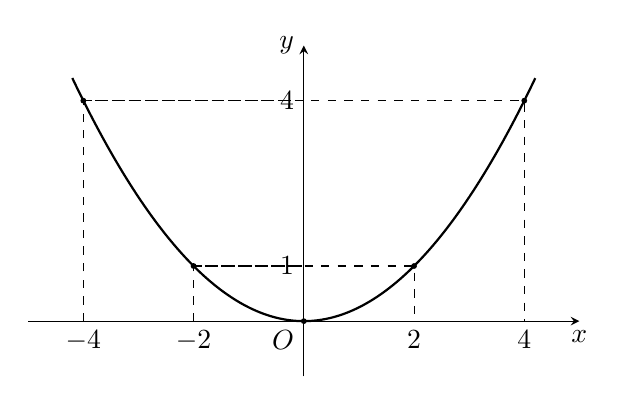
\begin{tikzpicture}[>=stealth,scale=0.7]
        \draw[->] (-5,0) -- (5,0) node[below] {$x$};
        \draw[->] (0,-1) -- (0,5) node[left] {$y$};
        \node[below left] at (0,0) {$O$};
        \draw[dashed] (-4,0) node[below] {$-4$} -- (-4,4) -- (4,4) -- (4,0) node[below] {$4$};
        \draw[dashed] (-2,0) node[below] {$-2$} -- (-2,1) -- (2,1) -- (2,0) node[below] {$2$};
        \draw[dashed] (-4,4) -- (0,4) node[left] {$4$};
        \draw[dashed] (-2,1) -- (0,1) node[left] {$1$};
        \draw[thick,smooth,samples=100,domain=-4.2:4.2] plot(\x,{0.25*(\x)^2});
        \fill (-4,4) circle (1.5pt) (-2,1) circle (1.5pt) (0,0) circle (1.5pt) (2,1) circle (1.5pt) (4,4) circle (1.5pt);
    \end{tikzpicture}
    \end{center}
    \item Điểm $M$ thuộc $(P)$ có tung độ bằng hai lần hoành độ nên thỏa mãn $y = 2x$.\\
    Ta có phương trình hoành độ giao điểm:
    $$2x = \dfrac{x^2}{4} \iff \dfrac{x^2}{4} - 2x = 0 \iff x(x - 8) = 0 \iff \left[\begin{aligned} &x = 0 \\ &x = 8. \end{aligned}\right.$$
    \begin{itemize}
        \item Với $x = 0 \implies y = 0$.
        \item Với $x = 8 \implies y = 2 \cdot 8 = 16$.
    \end{itemize}
    Vậy tọa độ các điểm cần tìm là $(0;0)$ và $(8;16)$.
\end{enumerate}
}
\end{bt}

\begin{bt}%[9D6H20-2]
% nguon: Cụm 12 – Đề tham khảo Tuyển sinh 10 năm học 2026-2027 TP.HCM – Đề số 34
Cho phương trình $2x^2 - 9x + 3 = 0$.
\begin{enumerate}[a)]
    \item Chứng tỏ phương trình luôn có hai nghiệm phân biệt $x_1, x_2$.
    \item Không giải phương trình, hãy tính giá trị của biểu thức:
    $$M = x_1(2025 - x_1) + x_2(2026 - x_2) - x_2.$$
\end{enumerate}
\loigiai{
\begin{enumerate}[a)]
    \item Phương trình $2x^2 - 9x + 3 = 0$ có $a = 2, b = -9, c = 3$.\\
    Ta có $\Delta = (-9)^2 - 4 \cdot 2 \cdot 3 = 81 - 24 = 57 > 0$.\\
    Vì $\Delta > 0$ nên phương trình luôn có hai nghiệm phân biệt $x_1, x_2$.
    \item Theo định lý Vi-ét, ta có:
    $$\begin{cases} x_1 + x_2 = \dfrac{9}{2} \\ x_1 x_2 = \dfrac{3}{2}. \end{cases}$$
    Ta có $x_1^2 + x_2^2 = (x_1 + x_2)^2 - 2x_1 x_2 = \left(\dfrac{9}{2}\right)^2 - 2 \cdot \dfrac{3}{2} = \dfrac{81}{4} - 3 = \dfrac{69}{4}$.\\
    Biến đổi biểu thức $M$:
    $$\begin{aligned}
    M &= 2025x_1 - x_1^2 + 2026x_2 - x_2^2 - x_2 \\
    &= 2025x_1 + 2025x_2 - (x_1^2 + x_2^2) \\
    &= 2025(x_1 + x_2) - (x_1^2 + x_2^2).
    \end{aligned}$$
    Thay $x_1 + x_2 = \dfrac{9}{2}$ và $x_1^2 + x_2^2 = \dfrac{69}{4}$ vào biểu thức, ta được:
    $$M = 2025 \cdot \dfrac{9}{2} - \dfrac{69}{4} = \dfrac{36450}{4} - \dfrac{69}{4} = \dfrac{36381}{4}.$$
\end{enumerate}
}
\end{bt}

\begin{bt}%[9D8H26-3]
% nguon: Cụm 12 – Đề tham khảo Tuyển sinh 10 năm học 2026-2027 TP.HCM – Đề số 34
Trong một nhóm gồm $10$ học sinh lớp 9 có $5$ bạn học trường THCS Quang Trung, $3$ bạn học trường THCS Nguyễn Huệ và $2$ bạn học trường THCS Tây Sơn. Chọn ngẫu nhiên $1$ bạn học sinh trong nhóm.
\begin{enumerate}[a)]
    \item Xác định số phần tử của không gian mẫu.
    \item Tính xác suất của mỗi biến cố sau:
    \begin{itemize}
        \item $A$: ``Bạn học sinh được chọn học trường THCS Quang Trung''.
        \item $B$: ``Bạn học sinh được chọn không học trường THCS Tây Sơn''.
    \end{itemize}
\end{enumerate}
\loigiai{
\begin{enumerate}[a)]
    \item Phép thử là chọn ngẫu nhiên $1$ bạn học sinh từ nhóm $10$ học sinh, nên số phần tử của không gian mẫu là $n(\Omega) = 10$.
    \item Tính xác suất của các biến cố:
    \begin{itemize}
        \item Có $5$ bạn học trường Quang Trung, nên số kết quả thuận lợi cho biến cố $A$ là $n(A) = 5$.\\
        Xác suất của biến cố $A$ là:
        $$P(A) = \dfrac{n(A)}{n(\Omega)} = \dfrac{5}{10} = \dfrac{1}{2}.$$
        \item Số bạn không học trường Tây Sơn là $10 - 2 = 8$ (bạn).\\
        Số kết quả thuận lợi cho biến cố $B$ là $n(B) = 8$.\\
        Xác suất của biến cố $B$ là:
        $$P(B) = \dfrac{n(B)}{n(\Omega)} = \dfrac{8}{10} = \dfrac{4}{5}.$$
    \end{itemize}
\end{enumerate}
}
\end{bt}

\begin{bt}%[9D6V21-3]
% nguon: Cụm 12 – Đề tham khảo Tuyển sinh 10 năm học 2026-2027 TP.HCM – Đề số 34
Một mảnh vườn hình chữ nhật có chiều rộng là $a\text{ (m)}$ và chiều dài hơn chiều rộng là $6\text{ m}$. Người ta làm hai lối đi chữ thập cắt nhau, mỗi lối đi rộng $x\text{ (m)}$ (với $0 < x < a$).
\begin{enumerate}[a)]
    \item Viết biểu thức theo $a$ và $x$ biểu thị diện tích phần đất còn lại dùng để trồng cây.
    \item Tính diện tích phần đất còn lại khi $a = 30\text{ m}$ và $x = 1\text{ m}$.
\end{enumerate}
\loigiai{
\begin{enumerate}[a)]
    \item Chiều rộng ban đầu của mảnh vườn là $a\text{ (m)}$.\\
    Chiều dài ban đầu của mảnh vườn là $a + 6\text{ (m)}$.\\
    Sau khi làm hai lối đi rộng $x\text{ (m)}$, bốn góc vườn còn lại có thể ghép lại thành một hình chữ nhật mới có:
    \begin{itemize}
        \item Chiều rộng là: $a - x\text{ (m)}$.
        \item Chiều dài là: $(a + 6) - x = a + 6 - x\text{ (m)}$.
    \end{itemize}
    Biểu thức diện tích phần đất còn lại của mảnh vườn là:
    $$S = (a - x)(a + 6 - x)\text{ (m}^2\text{)}.$$
    \item Khi $a = 30\text{ m}$ và $x = 1\text{ m}$, ta có diện tích phần đất còn lại là:
    $$S = (30 - 1)(30 + 6 - 1) = 29 \cdot 35 = 1015\text{ (m}^2\text{)}.$$
\end{enumerate}
}
\end{bt}

\begin{bt}%[9H0V31-3]
% nguon: Cụm 12 – Đề tham khảo Tuyển sinh 10 năm học 2026-2027 TP.HCM – Đề số 34
Một chiếc bình chứa nước dạng hình trụ có đường kính đáy là $8\text{ cm}$. Khi đặt bình thẳng đứng, mực nước trong bình cao $10\text{ cm}$. Khi úp ngược bình lại, phần không gian trống phía trên đỉnh bình có dạng hình trụ với chiều cao là $15\text{ cm}$.
\begin{enumerate}[a)]
    \item Tính thể tích nước có trong bình (làm tròn kết quả đến chữ số thập phân thứ hai).
    \item Nếu dùng bình này đựng đầy nước rồi rót vào các chiếc ly hình lập phương cạnh $4\text{ cm}$ thì rót đầy tối đa được bao nhiêu ly?
\end{enumerate}
Biết thể tích hình trụ là $V = \pi r^2 h$ ($r$ là bán kính đáy, $h$ là chiều cao) và thể tích hình lập phương là $V = s^3$ ($s$ là độ dài cạnh).
\loigiai{
\begin{enumerate}[a)]
    \item Bán kính đáy của bình hình trụ là:
    $$r = 8 : 2 = 4\text{ (cm)}.$$
    Thể tích nước có trong bình là:
    $$V_{\text{nước}} = \pi r^2 h_1 = \pi \cdot 4^2 \cdot 10 = 160\pi \approx 502{,}65\text{ (cm}^3\text{)}.$$
    \item Khi úp ngược bình, phần không gian trống có dạng hình trụ với bán kính đáy $r = 4\text{ cm}$ và chiều cao $h_2 = 15\text{ cm}$.\\
    Thể tích phần không gian trống trong bình là:
    $$V_{\text{trống}} = \pi r^2 h_2 = \pi \cdot 4^2 \cdot 15 = 240\pi\text{ (cm}^3\text{)}.$$
    Tổng dung tích của bình khi chứa đầy nước là:
    $$V_{\text{bình}} = V_{\text{nước}} + V_{\text{trống}} = 160\pi + 240\pi = 400\pi\text{ (cm}^3\text{)}.$$
    Thể tích của một ly hình lập phương cạnh $4\text{ cm}$ là:
    $$V_{\text{ly}} = 4^3 = 64\text{ (cm}^3\text{)}.$$
    Số ly nước rót được tối đa là:
    $$\dfrac{V_{\text{bình}}}{V_{\text{ly}}} = \dfrac{400\pi}{64} \approx 19{,}63\text{ (ly)}.$$
    Vì yêu cầu rót đầy ly nên số ly nước rót đầy tối đa là $19$ ly.
\end{enumerate}
}
\end{bt}

\begin{bt}%[9D1H3-4]
% nguon: Cụm 12 – Đề tham khảo Tuyển sinh 10 năm học 2026-2027 TP.HCM – Đề số 34
Theo kế hoạch, hai tổ công nhân phải sản xuất tổng cộng $700$ sản phẩm trong một thời gian nhất định. Nhờ áp dụng cải tiến kỹ thuật, tổ I đã làm vượt mức $12\%$ kế hoạch, trong khi tổ II giảm $5\%$ so với kế hoạch ban đầu. Tuy vậy, tính chung cả hai tổ vẫn hoàn thành vượt mức $16$ sản phẩm so với dự kiến. Hỏi theo kế hoạch ban đầu, mỗi tổ phải sản xuất bao nhiêu sản phẩm và thực tế số sản phẩm tổ I vượt mức là bao nhiêu?
\loigiai{
Gọi $x$ và $y$ (sản phẩm) lần lượt là số sản phẩm tổ I và tổ II phải sản xuất theo kế hoạch ($x, y \in \mathbb{N}^*, x, y < 700$).\\
Vì theo kế hoạch hai tổ phải sản xuất $700$ sản phẩm nên ta có phương trình:
$$x + y = 700 \quad (1)$$
Thực tế:
\begin{itemize}
    \item Tổ I vượt mức $12\%$ kế hoạch, tức làm thêm được: $12\% x = 0{,}12x$ (sản phẩm).
    \item Tổ II giảm $5\%$ kế hoạch, tức giảm: $5\% y = 0{,}05y$ (sản phẩm).
\end{itemize}
Vì cả hai tổ hoàn thành vượt mức $16$ sản phẩm nên ta có phương trình:
$$0{,}12x - 0{,}05y = 16 \quad (2)$$
Từ $(1)$ và $(2)$ ta có hệ phương trình:
$$\begin{cases} x + y = 700 \\ 0{,}12x - 0{,}05y = 16 \end{cases} \iff \begin{cases} 0{,}05x + 0{,}05y = 35 \\ 0{,}12x - 0{,}05y = 16 \end{cases} \iff \begin{cases} 0{,}17x = 51 \\ x + y = 700 \end{cases} \iff \begin{cases} x = 300 \\ y = 400 \end{cases}\text{ (thỏa mãn)}.$$
Số sản phẩm vượt mức của tổ I là:
$$300 \cdot 12\% = 36\text{ (sản phẩm)}.$$
Số sản phẩm bị giảm của tổ II là:
$$400 \cdot 5\% = 20\text{ (sản phẩm)}.$$
Vậy theo kế hoạch tổ I phải sản xuất $300$ sản phẩm, tổ II phải sản xuất $400$ sản phẩm; thực tế tổ I đã làm vượt mức $36$ sản phẩm.
}
\end{bt}

\begin{bt}%[9H9C29-3]
% nguon: Cụm 12 – Đề tham khảo Tuyển sinh 10 năm học 2026-2027 TP.HCM – Đề số 34
Cho đường tròn $(O; R)$ có đường kính $AB$. Vẽ hai tiếp tuyến $Ax, By$ với $(O)$. Điểm $E$ thuộc tia đối của tia $AB$ sao cho $A$ là trung điểm của đoạn thẳng $EO$. Từ $E$ kẻ tiếp tuyến $EM$ với đường tròn $(O)$ ($M$ là tiếp điểm), tiếp tuyến này cắt $Ax$ tại $C$ và cắt $By$ tại $D$.
\begin{enumerate}[a)]
    \item Chứng minh tứ giác $OMDB$ nội tiếp một đường tròn.
    \item Đoạn thẳng $AM$ cắt $OC$ tại $I$, đoạn thẳng $MB$ cắt $OD$ tại $K$. Chứng minh tứ giác $OKMI$ là hình chữ nhật và $\triangle OKI \backsim \triangle OCD$.
    \item Tính diện tích tứ giác $KICD$ theo $R$.
\end{enumerate}
\loigiai{
\begin{center}
\begin{tikzpicture}[scale=0.95]
    \coordinate (O) at (0,0);
    \def\R{2.2}
    \coordinate (A) at (-\R,0);
    \coordinate (B) at (\R,0);
    \draw[thick] (A) -- (B);
    \draw (O) circle (\R);
    \coordinate (E) at ({-2*\R},0); % A là trung điểm EO => E(-2R, 0)
    % Tiếp tuyến EM từ E: EO = 2R, OM = R => góc EOM = 60 độ
    \coordinate (M) at ({cos(60)*\R},{sin(60)*\R});
    \draw[dashed] (E) -- (A);
    \draw[thick] (E) -- (M);
    % C là giao điểm EM với tiếp tuyến Ax tại A: x = -R
    \coordinate (C) at (-\R,{ \R*tan(30) });
    % D là giao điểm EM với tiếp tuyến By tại B: x = R
    \coordinate (D) at (\R,{ \R*sqrt(3) });
    \draw[thick] (A) -- (C);
    \draw[thick] (B) -- (D);
    \draw[thick] (C) -- (D);
    \draw[dashed] (O) -- (C) (O) -- (D) (O) -- (M);
    \coordinate (I) at ($(A)!0.5!(M)$);
    \coordinate (K) at ($(B)!0.5!(M)$);
    \draw[thick] (A) -- (M) -- (B);
    \draw[thick,blue] (I) -- (K);
    \node[below] at (O) {$O$};
    \node[below left] at (A) {$A$};
    \node[below right] at (B) {$B$};
    \node[below left] at (E) {$E$};
    \node[above] at (M) {$M$};
    \node[left] at (C) {$C$};
    \node[right] at (D) {$D$};
    \node[below left] at (I) {$I$};
    \node[below right] at (K) {$K$};
    \fill (O) circle (1.5pt) (A) circle (1.5pt) (B) circle (1.5pt) (E) circle (1.5pt) (M) circle (1.5pt) (C) circle (1.5pt) (D) circle (1.5pt) (I) circle (1.5pt) (K) circle (1.5pt);
\end{tikzpicture}
\end{center}
\begin{enumerate}[a)]
    \item Vì $MD$ và $BD$ là các tiếp tuyến của $(O)$ tại $M$ và $B$ nên $\widehat{OMD} = \widehat{OBD} = 90^\circ$.\\
    Tứ giác $OMDB$ có hai đỉnh kề $M, B$ cùng nhìn đoạn $OD$ dưới một góc $90^\circ$ (hoặc $\widehat{OMD} + \widehat{OBD} = 180^\circ$) nên nội tiếp đường tròn đường kính $OD$.
    \item Ta có $CA = CM$ (tính chất hai tiếp tuyến cắt nhau) và $OA = OM = R$, nên $OC$ là đường trung trực của đoạn thẳng $AM \implies OC \perp AM$ tại $I$, do đó $\widehat{OIM} = 90^\circ$.\\
    Tương tự, $DB = DM$ và $OB = OM = R$ nên $OD$ là đường trung trực của đoạn thẳng $BM \implies OD \perp BM$ tại $K$, do đó $\widehat{OKM} = 90^\circ$.\\
    Mặt khác, $\widehat{AMB} = 90^\circ$ (góc nội tiếp chắn nửa đường tròn đường kính $AB$).\\
    Tứ giác $OKMI$ có ba góc vuông: $\widehat{OIM} = \widehat{OKM} = \widehat{IMK} = 90^\circ$ nên là hình chữ nhật.\\
    Trong tam giác vuông $OMC$ có đường cao $MI$:
    $$OM^2 = OI \cdot OC.$$
    Trong tam giác vuông $OMD$ có đường cao $MK$:
    $$OM^2 = OK \cdot OD.$$
    Suy ra $OI \cdot OC = OK \cdot OD \implies \dfrac{OK}{OC} = \dfrac{OI}{OD}$.\\
    Xét $\triangle OKI$ và $\triangle OCD$ có:
    $$\widehat{COD}\text{ chung, } \dfrac{OK}{OC} = \dfrac{OI}{OD}.$$
    Suy ra $\triangle OKI \backsim \triangle OCD$ (c-g-c).
    \item Vì $A$ là trung điểm của $EO$ nên $EO = 2OA = 2R$.\\
    Tam giác vuông $EMO$ tại $M$ có $\cos \widehat{EOM} = \dfrac{OM}{EO} = \dfrac{R}{2R} = \dfrac{1}{2} \implies \widehat{EOM} = 60^\circ$.\\
    Do đó $\widehat{AOM} = 60^\circ \implies \widehat{MOB} = 180^\circ - 60^\circ = 120^\circ$.\\
    Theo tính chất hai tiếp tuyến cắt nhau, ta có:
    $$\widehat{AOC} = \widehat{MOC} = \dfrac{1}{2}\widehat{AOM} = 30^\circ,$$
    $$\widehat{BOD} = \widehat{MOD} = \dfrac{1}{2}\widehat{MOB} = 60^\circ.$$
    Suy ra $\widehat{COD} = \widehat{MOC} + \widehat{MOD} = 30^\circ + 60^\circ = 90^\circ$.\\
    Trong tam giác vuông $OAC$ tại $A$:
    $$OC = \dfrac{OA}{\cos 30^\circ} = \dfrac{R}{\dfrac{\sqrt{3}}{2}} = \dfrac{2R\sqrt{3}}{3}.$$
    Trong tam giác vuông $OBD$ tại $B$:
    $$OD = \dfrac{OB}{\cos 60^\circ} = \dfrac{R}{\dfrac{1}{2}} = 2R.$$
    Diện tích tam giác vuông $OCD$ là:
    $$S_{OCD} = \dfrac{1}{2} \cdot OC \cdot OD = \dfrac{1}{2} \cdot \dfrac{2R\sqrt{3}}{3} \cdot 2R = \dfrac{2R^2\sqrt{3}}{3}.$$
    Ta có $OI = \dfrac{OM^2}{OC} = \dfrac{R^2}{\dfrac{2R\sqrt{3}}{3}} = \dfrac{R\sqrt{3}}{2}$.\\
    Tỉ số đồng dạng của $\triangle OKI$ và $\triangle OCD$ là:
    $$k = \dfrac{OI}{OD} = \dfrac{\dfrac{R\sqrt{3}}{2}}{2R} = \dfrac{\sqrt{3}}{4}.$$
    Suy ra diện tích tam giác $OKI$ là:
    $$S_{OKI} = k^2 \cdot S_{OCD} = \left(\dfrac{\sqrt{3}}{4}\right)^2 \cdot \dfrac{2R^2\sqrt{3}}{3} = \dfrac{3}{16} \cdot \dfrac{2R^2\sqrt{3}}{3} = \dfrac{R^2\sqrt{3}}{8}.$$
    Diện tích tứ giác $KICD$ là:
    $$S_{KICD} = S_{OCD} - S_{OKI} = \dfrac{2R^2\sqrt{3}}{3} - \dfrac{R^2\sqrt{3}}{8} = \dfrac{16R^2\sqrt{3} - 3R^2\sqrt{3}}{24} = \dfrac{13R^2\sqrt{3}}{24}.$$
\end{enumerate}
}
\end{bt}
